\chapter{Resultados}
\label{chap:resultados}
Este capítulo irá mostrar os resultados da comparação dos sistemas criados, um que utiliza a persistência monoglota e outro que utiliza a persistência poliglota. O modelo de persistência poliglota tinha como alvo melhorar o desempenho da página \verb|feed|, mas sabemos que para isso a escrita do \textit{tweet} iria ser mais lenta. Pois, ao usuário publicar o \textit{tweet} é necessário atualizar a \textit{feed} de todos os seguidores desse usuário. Então iremos comparar o tempo de consulta da \textit{feed} de \textit{tweets} e o tempo de inserção de um \textit{tweet}. 

O capítulo foi dividido em três seções, a \autoref{sec:resultFeed} que descreve como foram feito os testes para medir tempo de consulta da \textit{feed} de \textit{tweets}, a \autoref{sec:resultInsertTweet} descreve como foram feito os testes para medir o tempo de inserção de um \textit{tweet} e a \autoref{sec:resultEval} irá analisar os resultados encontrados.

Para medir o tempo das operações utilizamos uma classe do próprio \textit{Ruby}, chamada \textit{Benchmark} \footnote{A documentação da classe Benchmark. \url{http://www.ruby-doc.org/stdlib-2.0/libdoc/benchmark/rdoc/Benchmark.html}}. Dessa classe utilizamos o método chamado \textit{measure} que mede o tempo de execução. Esse tempo medido está incluído o tempo da operação no banco de dados e o tempo do carregamento dos valores para as variáveis do sistema.

Os testes foram realizados na máquina Asus, modelo N82J\footnote{A especificação se encontra no sítio da Asus \url{http://www.asus.com/Notebooks_Ultrabooks/N82Jq/}}, porém foi adicionado, nessa máquina, mais 4GB de RAM e o sistema operacional é Ubuntu 14.04 LTS.


\section{Resultados do tempo de consulta da \textit{feed} de \textit{tweets}}
\label{sec:resultFeed}

Para fazer um teste, no qual esses tempos medidos resultassem em uma diferença significativa criamos quatro bancos de dados do MongoDB. Esses bancos foram populados com cem usuários, porém a diferença entre os bancos foi a quantidade de \textit{tweets} de cada usuário. No primeiro banco de dados foi adicionado dez \textit{tweets} para cada usuário, totalizando em mil \textit{tweets}, no segundo foram adicionados cem \textit{tweets} para cada usuário, totalizando em dez mil \textit{tweets}, no terceiro banco foram adicionados mil \textit{tweets} para cada usuário totalizando em cem mil \textit{tweets} e, por último, foram adicionados, no quarto banco de dados, dez mil \textit{tweets} para cada usuário, totalizando em um milhão de \textit{tweets}.

Alteramos o primeiro usuário para seguir todos os outros noventa e nove usuários e executamos o método \verb|remake_feed| da classe \verb|User| para criar a chave no \ac{Redis}.

No modelo monoglota medimos o tempo de execução da seguinte função:
\begin{lstlisting}
Tweet.in(user_id: user.following_ids).desc("created_at").
      paginate(:page => 1, :per_page => 100)
\end{lstlisting}

Essa função irá buscar os cem \textit{tweets} mais recentes que o usuário atribuído ao objeto \textit{user} segue. Repetimos a execução dessa função cem vezes para cada banco de dados, que havíamos populado. Fizemos a média das cem repetições para cada banco e colocamos os valores em um gráfico e uma tabela para fazer a análise:

\begin{figure}[H]
    \centering
    \caption{Tempo de consulta da \textit{feed} de \textit{tweets} com persisência monoglota}
    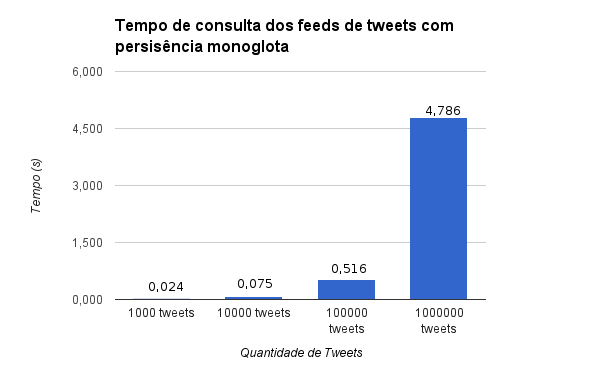
\includegraphics[width=0.8\textwidth]{./04-figuras/time_feed_mono.png}
    \fonte{Autoria Própria}
    \label{fig:time_feed_mono}
\end{figure}

\begin{table}[H]
    \centering
    \caption[Tempo médio de consulta da feed de Tweets com persistência monoglota]{Tempo médio de consulta da feed de Tweets com persistência monoglota.\label{tab:tempo_feed_mono}}
    \begin{tabular}{ccc}
        \hline
            Quantidade de \textit{Tweets} & Tempo (s) \\
        \hline
            1000 \textit{tweets} &   0,02367260216 \\
            10.000 \textit{tweets} & 0,07490080889 \\
            100.000 \textit{tweets} & 0,51625828603 \\
            1.000.000 \textit{tweets} & 4,78559743231 \\
        \hline
    \end{tabular}
    \fonte{Autoria própria.}
\end{table}



Podemos observar que o aumento da quantidade de \textit{tweets} foi quase diretamente proporcional com o tempo gasto.


No modelo poliglota medimos o tempo de execução da seguinte função: 
\begin{lstlisting}
	Tweet.feed_of user
\end{lstlisting} 

Essa função busca no \ac{Redis} a chave do usuário \textit{user} que contém os cem \textit{tweets} mais recentes que esse usuário segue. Também medimos cem vezes para cada banco de dados, que havíamos populado. Segue abaixo o gráfico com a média do tempo executado para cada banco de dados:

\begin{figure}[H]
    \centering
    \caption{Tempo de consulta da \textit{feed} de \textit{tweets} com persisência poliglota}
    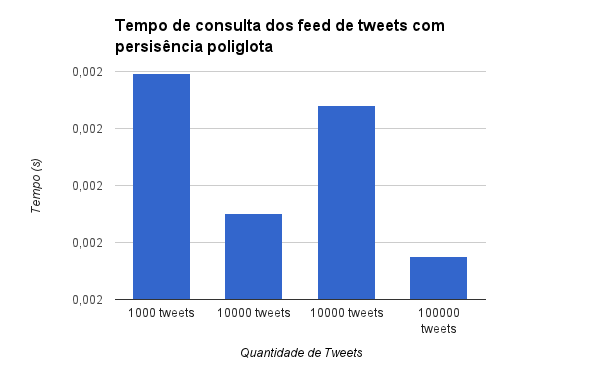
\includegraphics[width=0.8\textwidth]{./04-figuras/time_feed_poli.png}
    \fonte{Autoria Própria}
    \label{fig:time_feed_poli}
\end{figure}

\begin{table}[H]
    \centering
    \caption[Tempo médio de consulta da feed de Tweets com persistência poliglota]{Tempo médio de consulta da feed de Tweets com persistência poliglota.\label{tab:tempo_feed_poli}}
    \begin{tabular}{ccc}
        \hline
            Quantidade de \textit{Tweets} & Tempo (s) \\
        \hline
            1000 \textit{tweets} &   0,00203783201 \\
            10.000 \textit{tweets} & 0,00189030516 \\
            100.000 \textit{tweets} & 0,00200452554 \\
            1.000.000 \textit{tweets} & 0,00184512174 \\
        \hline
    \end{tabular}
    \fonte{Autoria própria.}
\end{table}


Podemos observar que o tempo varia um pouco com as diferentes quantidades de \textit{tweets}, mas não é proporcional à quantidade de \textit{tweets}.

\section{Resultados do tempo de inserção de um \textit{tweet}}
\label{sec:resultInsertTweet}
Para realizar os testes de inserção de um \textit{tweet} criamos um banco de dados MongoDB com dez mil e um usuários, cada usuário com cem \textit{tweets}, totalizando em mais de um milhão de \textit{tweets} e rodamos o método \verb|remake_feed| para polular o \ac{Redis}. 

Alteramos a quantidade de seguidores do ultimo usuário para cem, mil, e dez mil seguidores e para cada conjunto de seguidores inserimos um \textit{tweet} cem vezes e medimos o tempo de cada inserção.

Para medir esse tempo de inserção em ambos os sistemas utilizamos a mesma função. A diferença da persistência poliglota é que foi criado um \textit{call back} que é executado após o \textit{tweet} ser criado. Esse \textit{call back} realiza uma operação de leitura e outra de escrita no \ac{Redis} para cada seguidor. Ou seja, na implementação poliglota a cada \textit{tweet} inserido por um usuário, a chave de todos os seguidores desse usuário é refeita no \ac{Redis}. 

Para a persistência monoglota obtivemos os seguintes resultados:

\begin{figure}[H]
    \centering
    \caption{Tempo de inserção de um \textit{tweet} com persisência monoglota}
    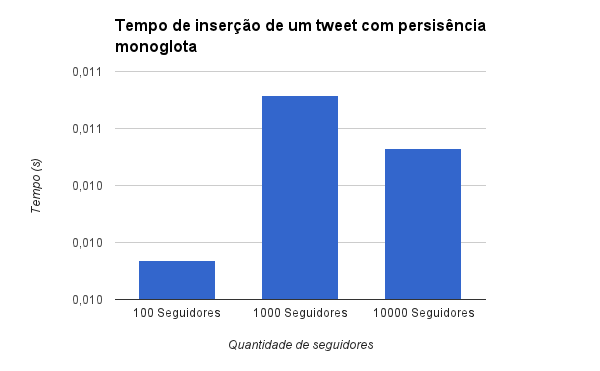
\includegraphics[width=0.8\textwidth]{./04-figuras/insert_mono.png}
    \fonte{Autoria Própria}
    \label{fig:insert_mono}
\end{figure}

\begin{table}[H]
    \centering
    \caption[Tempo médio de inserção \textit{tweet} com persistência monoglota]{Tempo médio de inserção \textit{tweet} com persistência monoglota.\label{tab:insert_mono}}
    \begin{tabular}{ccc}
        \hline
            Quantidade de seguidores & Tempo (s) \\
        \hline
            100  &   0,01013553935 \\
            1.000  & 0,01071643248 \\
            10.000 & 0,01052849981 \\
        \hline
    \end{tabular}
    \fonte{Autoria própria.}
\end{table}


Já para a persistência poliglota, construímos dois gráficos, um que mostra o tempo total gasto para cada conjunto de seguidores e outro que mostra o valor percentual do tempo gasto pelo MongoDB. Colocamos a tabela para podermos exibir o valor encontrado.

\begin{figure}[H]
    \centering
    \caption{Tempo de inserção de um \textit{tweet} com persisência poliglota}
    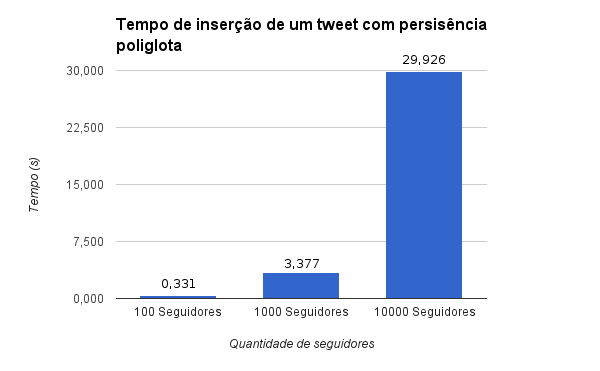
\includegraphics[width=0.8\textwidth]{./04-figuras/insert_poli.png}
    \fonte{Autoria Própria}
    \label{fig:insert_poli}
\end{figure}

\begin{table}[H]
    \centering
    \caption[Tempo médio de inserção \textit{tweet} com persistência poliglota]{Tempo médio de inserção \textit{tweet} com persistência poliglota.\label{tab:insert_poli}}
    \begin{tabular}{ccc}
        \hline
            Quantidade de seguidores & Tempo (s) \\
        \hline
            100  &   0,3313111267 \\
            1.000  & 3,37695235061 \\
            10.000 & 29,92647902573 \\
        \hline
    \end{tabular}
    \fonte{Autoria própria.}
\end{table}


\begin{figure}[H]
    \centering
    \caption{Porcentagem do tempo gasto pelo MongoDB}
    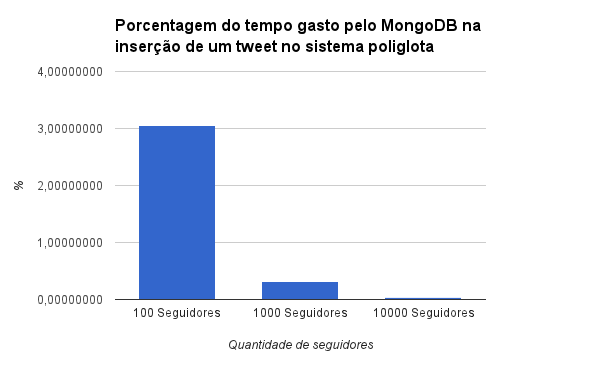
\includegraphics[width=0.8\textwidth]{./04-figuras/percent_mongo.png}
    \fonte{Autoria Própria}
    \label{fig:percent_mongo}
\end{figure}

\begin{table}[H]
    \centering
    \caption[Porcentagem do tempo gasto pelo MongoDB]{Porcentagem do tempo gasto pelo MongoDB.\label{tab:percent_mongo}}
    \begin{tabular}{ccc}
        \hline
            Quantidade de seguidores & \% \\
        \hline
            100  &   3,05922094 \\
            1.000  & 0,31734035 \\
            10.000 & 0,03518122 \\
        \hline
    \end{tabular}
    \fonte{Autoria própria.}
\end{table}


\section{Análise dos resultados}
\label{sec:resultEval}

Para a implementação monoglota tivemos piores resultados na consulta a \textit{feed} de \textit{tweets}. A média aumentou significativamente quando a quantidade de \textit{tweets} no banco foram aumentados. Isso era esperado acontecer, pois para o banco encontrar os documentos procurados, foi necessário percorrer todos os \textit{tweets} e comparar com os parâmetros passados na consulta.
Já para a implementação poliglota, o tempo de execução para as diferentes quantidades de \textit{tweets} foram muito próximos, pois a consulta é apenas para buscar a chave, não há nenhuma outra comparação ou leitura a ser feita. Isso pode ser comprovado comparando as tabelas \ref{tab:tempo_feed_mono} e \ref{tab:tempo_feed_poli}.
Com isso, podemos observar que tivemos uma melhora significativa, pois em nenhum momento a consulta a \textit{feed} de \textit{tweets} de um usuário foi mais rápida no sistema monoglota.

Em relação aos resultados do tempo de inserção do \textit{tweet}, podemos observar que em nenhum instante a implementação poliglota foi mais rápida. Isso é devido ao tempo que foi gasto para atualizar as chaves. O aumento de seguidores foi proporcional com o aumento do tempo, ou seja, se aumentarmos em dez vezes os seguidores o tempo de atualização das chaves será dez vezes maior. A \autoref{tab:percent_mongo} mostra que com o aumento de seguidores o percentual de tempo gasto no MongoDB se torna menor e consequentemente o tempo gasto com o \ac{Redis} maior.
Isso porque precisamos de fazer uma leitura e uma escrita para cada chave ser atualizada, ou seja, operações no \ac{Redis}. Já para a implementação monoglota não houve diferença, pois a inserção de um \textit{tweet} não depende da quantidade de seguidores e está apenas vinculada ao MongoDB.


